\documentclass[11pt]{article}

\usepackage[margin=1in]{geometry}
\usepackage{amsmath,amssymb,amsthm}
\usepackage{tikz}
\usetikzlibrary{positioning,arrows.meta,calc,decorations.pathreplacing}
\usepackage{hyperref}
\usepackage{enumitem}
\usepackage{microtype}
\usepackage{algorithm}
\usepackage{algpseudocode}

\theoremstyle{plain}
\newtheorem{theorem}{Theorem}[section]
\newtheorem{lemma}[theorem]{Lemma}
\newtheorem{corollary}[theorem]{Corollary}
\newtheorem{proposition}[theorem]{Proposition}

\theoremstyle{definition}
\newtheorem{definition}[theorem]{Definition}
\newtheorem{example}[theorem]{Example}

\theoremstyle{remark}
\newtheorem{remark}[theorem]{Remark}

% Notation shortcuts
\newcommand{\adj}{\operatorname{adj}}
\newcommand{\nodes}{\operatorname{nodes}}
\newcommand{\Mdomain}{\operatorname{dom}}
\newcommand{\Munion}{\operatorname{Munion}}
\newcommand{\nbs}{\operatorname{nbs}}
\newcommand{\degree}{\operatorname{deg}}
\newcommand{\maxdeg}{\operatorname{maxdeg}}
\newcommand{\restrict}{\operatorname{restrict}}
\newcommand{\Nat}{\mathbb{N}}
\newcommand{\Pos}{\mathbb{Z}^{+}}
\newcommand{\powerset}{\mathcal{P}}
\newcommand{\ie}{\textit{i.e.}}
\newcommand{\eg}{\textit{e.g.}}

\title{A Formal Proof of Wigderson's Graph Coloring Algorithm}
\author{}
\date{}

\begin{document}
\maketitle

\begin{abstract}
We present a complete formal verification of Wigderson's 1983 graph coloring algorithm in the Coq proof assistant.
The algorithm produces an $O(\!\sqrt{n})$-coloring of any 3-colorable graph on $n$ vertices.
Our development covers all the necessary infrastructure: an adjacency-list graph representation using positive maps and sets,
a greedy coloring algorithm, induced subgraphs, neighborhoods, independent sets, bipartiteness,
BFS-based 2-coloring of bipartite graphs, and both phases of Wigderson's algorithm.
The main results are: (1)~the algorithm produces a proper coloring of any 3-colorable undirected graph, (2)~every color assigned satisfies $c_i \le 3\lfloor n/(k{+}2)\rfloor + k + 2$, and (3)~setting $k = \lfloor\!\sqrt{n}\rfloor$ yields $c_i \le 4\sqrt{n} + 2$, formally establishing the $O(\!\sqrt{n})$ bound.
The formalization is approximately 6{,}600 lines of Coq, with extensive use of the CoqHammer automated tactic for proof automation.
No axioms beyond the standard Coq library are used, and no proofs are left admitted.
\end{abstract}

%% ====================================================================
\section{Introduction}
\label{sec:intro}

The graph coloring problem asks: given an undirected graph~$G$, assign colors to vertices so that no two adjacent vertices share a color.
The \emph{chromatic number}~$\chi(G)$ is the minimum number of colors needed.
Determining $\chi(G)$ is NP-hard in general, and even deciding whether $\chi(G) \le 3$ is NP-complete.

In 1983, Wigderson~\cite{wigderson83} observed that while \emph{finding} a 3-coloring is hard,
one can \emph{use} the existence of a 3-coloring to obtain an efficient algorithm that colors a 3-colorable graph
with $O(\!\sqrt{n})$ colors, where $n = |V(G)|$.
The key insight is that in any 3-colorable graph, the neighborhood of every vertex is 2-colorable (bipartite),
so the neighborhood of a high-degree vertex can be efficiently 2-colored, removing many vertices at once.

In this paper we present a complete formalization of this result in the Coq proof assistant.
Our development proceeds as follows:
\begin{enumerate}[nosep]
  \item We represent graphs as finite maps from vertices to adjacency sets, using Coq's \texttt{PositiveMap} and \texttt{PositiveSet} modules.
  \item We develop the theory of induced subgraphs, neighborhoods, degrees, and independent sets.
  \item We prove that a greedy coloring algorithm produces valid colorings.
  \item We formalize bipartiteness and prove the equivalence between bipartiteness and 2-colorability.
  \item We implement and verify a BFS-based 2-coloring algorithm for bipartite graphs.
  \item We implement both phases of Wigderson's algorithm, prove the main correctness theorem, and formally verify the $O(\!\sqrt{n})$ color bound.
\end{enumerate}

\begin{figure}[ht]
\centering
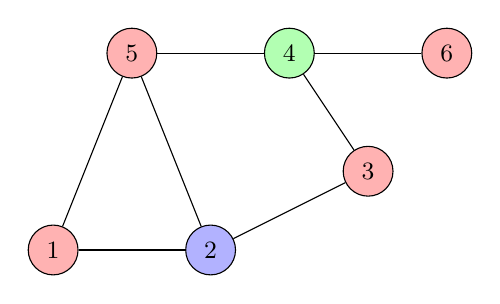
\begin{tikzpicture}[
  vertex/.style={circle, draw, minimum size=18pt, inner sep=0pt, font=\small},
  every edge/.style={draw, thick}
]
  % A small 3-colorable graph (6 vertices)
  \node[vertex, fill=red!30]   (1) at (0,0)    {1};
  \node[vertex, fill=blue!30]  (2) at (2,0)    {2};
  \node[vertex, fill=red!30]   (3) at (4,1)    {3};
  \node[vertex, fill=green!30] (4) at (3,2.5)  {4};
  \node[vertex, fill=red!30]   (5) at (1,2.5)  {5};
  \node[vertex, fill=red!30]   (6) at (5,2.5)  {6};

  \draw (1) -- (2);
  \draw (1) -- (5);
  \draw (2) -- (3);
  \draw (2) -- (5);
  \draw (3) -- (4);
  \draw (4) -- (5);
  \draw (4) -- (6);
\end{tikzpicture}
\caption{A small 3-colorable graph with a proper 3-coloring indicated by vertex shading.}
\label{fig:3coloring}
\end{figure}

%% ====================================================================
\section{Preliminaries: Graph Representation}
\label{sec:prelim}

\subsection{Core Definitions}

We represent graphs using Coq's \texttt{PositiveMap} and \texttt{PositiveSet} modules, which provide efficient finite maps and sets over the type of positive integers.

\begin{definition}[Graph]
A \emph{graph} is a finite map $g : \texttt{node} \to \texttt{nodeset}$, where $\texttt{node} = \Pos$ and $\texttt{nodeset} = \powerset_{\mathrm{fin}}(\Pos)$.
For a vertex $i$, its \emph{adjacency set} is
\[
  \adj(g, i) = \begin{cases} s & \text{if } g(i) = \texttt{Some}\; s, \\ \emptyset & \text{if } g(i) = \texttt{None}. \end{cases}
\]
The \emph{vertex set} (nodes) of $g$ is
$\nodes(g) = \Mdomain(g) = \{k \mid k \in \operatorname{dom}(g)\}$.
\end{definition}

\begin{definition}[Graph Properties]
A graph $g$ is:
\begin{itemize}[nosep]
  \item \emph{well-formed} if for all $i, j$: $j \in \adj(g, i) \implies j \in \operatorname{dom}(g)$.
  \item \emph{undirected} if for all $i, j$: $j \in \adj(g, i) \implies i \in \adj(g, j)$.
  \item \emph{irreflexive} (no self-loops) if for all $i$: $i \notin \adj(g, i)$.
\end{itemize}
\end{definition}

\begin{lemma}
\label{lem:undirected-wf}
Every undirected graph is well-formed.
\end{lemma}

\begin{proof}
If $j \in \adj(g, i)$ and $g$ is undirected, then $i \in \adj(g, j)$, which requires $g(j) = \texttt{Some}\; s$ for some $s$, hence $j \in \operatorname{dom}(g)$.
\end{proof}

\subsection{Colorings}

\begin{definition}[Coloring]
A \emph{coloring} is a finite map $f : \texttt{node} \to \texttt{node}$, assigning color values to vertices.
\end{definition}

\begin{definition}[Valid Coloring]
A coloring $f$ is \emph{valid} (or \emph{OK}) with respect to a palette $P$ and graph $g$ if for every edge $(i,j)$ in $g$:
\begin{enumerate}[nosep]
  \item if $f(i) = c_i$ then $c_i \in P$ (palette membership), and
  \item if $f(i) = c_i$ and $f(j) = c_j$ then $c_i \neq c_j$ (proper coloring).
\end{enumerate}
Formally: $\forall\, i\, j,\; j \in \adj(g,i) \implies (\forall c_i,\, f(i) = c_i \implies c_i \in P) \;\wedge\; (\forall c_i\, c_j,\, f(i)=c_i \implies f(j)=c_j \implies c_i \neq c_j)$.
\end{definition}

Note that this definition permits \emph{partial} colorings: vertices with $f(i) = \texttt{None}$ impose no constraint.

\begin{definition}[Complete Coloring, $n$-Coloring]
A coloring $f$ is \emph{complete} for $(P, g)$ if it is valid and every vertex of $g$ is colored: $\forall i,\; i \in \operatorname{dom}(g) \implies i \in \operatorname{dom}(f)$.

An \emph{$n$-coloring} is a coloring $f$ with a palette $P$ satisfying $|P| = n$ and every color used by $f$ belongs to $P$.
A \emph{three-coloring} is a 3-coloring; a \emph{two-coloring} is a 2-coloring.
\end{definition}

\begin{lemma}
\label{lem:complete-no-selfloop}
If $g$ admits a complete coloring, then $g$ has no self-loops.
\end{lemma}

\begin{lemma}
\label{lem:subgraph-coloring}
If $g'$ is a subgraph of $g$ and $f$ is a valid coloring of $g$, then $f$ is a valid coloring of $g'$.
\end{lemma}

%% ====================================================================
\section{Map Operations: Restriction and Union}
\label{sec:map-ops}

\subsection{Map Restriction}

\begin{definition}[Restriction]
For a map $m$ and a set $s$, the \emph{restriction} $\restrict(m, s)$ retains only the entries whose keys belong to $s$:
\[
  \restrict(m, s)(k) = \begin{cases} m(k) & \text{if } k \in s, \\ \texttt{None} & \text{otherwise}. \end{cases}
\]
This is implemented as $\texttt{WP.filter}\;(\lambda\,k\,v.\; k \in s)\;m$.
\end{definition}

\begin{lemma}[Restriction Characterization]
\label{lem:restrict-find}
$\restrict(m, s)(k) = \texttt{Some}\;v$ if and only if $k \in s$ and $m(k) = \texttt{Some}\;v$.
\end{lemma}

\begin{lemma}[Adjacency under Restriction]
\label{lem:adj-restrict}
For a graph $g$ and set $s$: $i \in \adj(\restrict(g,s), j) \iff i \in \adj(g,j) \wedge j \in s$.
\end{lemma}

\subsection{Map Union}

\begin{definition}[Left-Biased Map Union]
The \emph{union} of two maps $c$ and $d$, written $\Munion(c, d)$, is defined by folding insertion of all entries of $c$ into $d$:
$\Munion(c, d) = \texttt{fold}\;(\lambda\, k\, v\, m.\; m[k \mapsto v])\; c\; d$.
When both maps define a key, the left map's value takes priority.
\end{definition}

\begin{definition}[Map Disjointness]
Two maps $f, g$ are \emph{disjoint}, written $\texttt{Mdisjoint}(f, g)$, if
$\Mdomain(f) \cap \Mdomain(g) = \emptyset$.
\end{definition}

\begin{lemma}[Union Case Analysis]
\label{lem:munion-case}
If $\Munion(c,d)(i) = v$, then $c(i) = v$ or $d(i) = v$.
\end{lemma}

\begin{lemma}[Left Priority]
\label{lem:munion-find-l}
If $c(i) = v$, then $\Munion(c,d)(i) = v$.
\end{lemma}

\begin{lemma}[Union Membership]
\label{lem:munion-in}
$i \in \operatorname{dom}(\Munion(c,d)) \iff i \in \operatorname{dom}(c) \lor i \in \operatorname{dom}(d)$.
\end{lemma}

%% ====================================================================
\section{Subgraphs, Neighborhoods, and Independent Sets}
\label{sec:subgraph}

\subsection{Induced Subgraphs}

\begin{definition}[Induced Subgraph]
The \emph{induced subgraph} of $g$ on a vertex set $s$ is
\[
  \texttt{subgraph\_of}(g, s) = \texttt{map}\;(\lambda\, a.\; s \cap a)\;(\restrict(g, s)).
\]
This restricts both the vertex set and every adjacency set to $s$.
\end{definition}

\begin{definition}[Subgraph Predicate]
We write $\texttt{is\_subgraph}(g', g)$ when
$\nodes(g') \subseteq \nodes(g)$ and for all~$v$, $\adj(g', v) \subseteq \adj(g, v)$.
\end{definition}

\begin{lemma}[Adjacency in Induced Subgraphs]
$i \in \adj(\texttt{subgraph\_of}(g, s), j) \iff i \in \adj(g, j) \wedge i \in s \wedge j \in s$.
\end{lemma}

\begin{lemma}
$\texttt{subgraph\_of}(g, s)$ is a subgraph of $g$. Induced subgraphs preserve undirectedness.
\end{lemma}

\subsection{Node Removal}

\begin{definition}[Removing Nodes]
For a set $s$ of vertices to remove:
\[
  \texttt{remove\_nodes}(g, s) = \texttt{map}\;(\lambda\, a.\; a \setminus s)\;(\restrict(g, \nodes(g) \setminus s)).
\]
\end{definition}

\begin{lemma}[Adjacency after Removal]
\label{lem:adj-remove}
$i \in \adj(\texttt{remove\_nodes}(g,s), j) \iff i \in \adj(g,j) \wedge i \notin s \wedge j \notin s$.
\end{lemma}

\begin{lemma}
Removing a non-empty set of vertices that intersects $\operatorname{dom}(g)$ strictly decreases the graph's cardinality. Removal preserves undirectedness and irreflexivity.
\end{lemma}

\subsection{Neighborhoods}

\begin{definition}[Neighborhood]
The \emph{(open) neighborhood} of vertex $v$ in $g$ is the induced subgraph on $\adj(g,v)$, with $v$ itself removed:
\[
  \texttt{neighborhood}(g, v) = \texttt{remove\_node}(v, \texttt{subgraph\_of}(g, \adj(g,v))).
\]
\end{definition}

\begin{figure}[ht]
\centering
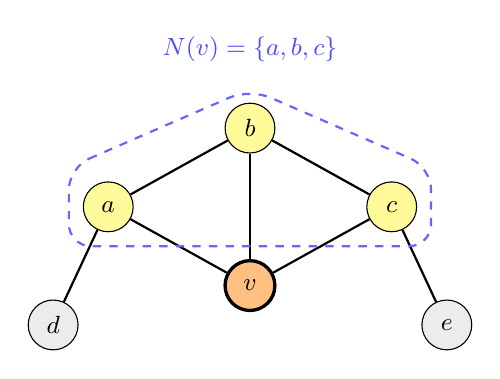
\begin{tikzpicture}[
  vertex/.style={circle, draw, minimum size=18pt, inner sep=0pt, font=\small},
  nbr/.style={vertex, fill=yellow!40},
  center/.style={vertex, fill=orange!50, very thick},
  other/.style={vertex, fill=gray!15}
]
  \node[center] (v) at (0,0)   {$v$};
  \node[nbr]    (a) at (-1.8,1)  {$a$};
  \node[nbr]    (b) at (0,2)   {$b$};
  \node[nbr]    (c) at (1.8,1)  {$c$};
  \node[other]  (d) at (-2.5,-0.5) {$d$};
  \node[other]  (e) at (2.5,-0.5)  {$e$};

  \draw[thick] (v) -- (a);
  \draw[thick] (v) -- (b);
  \draw[thick] (v) -- (c);
  \draw[thick] (a) -- (b);
  \draw[thick] (b) -- (c);
  \draw[thick] (a) -- (d);
  \draw[thick] (c) -- (e);

  % highlight neighborhood
  \draw[dashed, blue!60, thick, rounded corners=8pt]
    ($(a)+(-0.5,0.5)$) -- ($(b)+(0,0.5)$) -- ($(c)+(0.5,0.5)$) -- ($(c)+(0.5,-0.5)$) -- ($(a)+(-0.5,-0.5)$) -- cycle;
  \node[blue!70, font=\small] at (0,3) {$N(v) = \{a, b, c\}$};
\end{tikzpicture}
\caption{Vertex $v$ (orange) with its open neighborhood $N(v) = \{a, b, c\}$ (yellow, enclosed by dashed boundary). Edges within the neighborhood ($a$--$b$, $b$--$c$) form the induced subgraph. Vertices $d, e$ are outside.}
\label{fig:neighborhood}
\end{figure}

\begin{lemma}[Neighborhood Nodes]
\label{lem:nbd-nodes}
For an irreflexive undirected graph~$g$,
\[
  \nodes(\texttt{neighborhood}(g, v)) = \adj(g, v).
\]
\end{lemma}

\begin{lemma}
The neighborhood of $v$ is a subgraph of $g$ and inherits undirectedness.
\end{lemma}

\subsection{Degrees and Maximum Degree}

\begin{definition}[Degree, Maximum Degree]
The \emph{degree} of $v$ in $g$ is $\degree(v, g) = |\adj(g,v)|$ (when $v \in g$). The \emph{maximum degree} is $\maxdeg(g) = \max_{v \in g} \degree(v, g)$.
\end{definition}

\begin{lemma}
For any vertex $v$ with adjacency set $e$: $|e| \le \maxdeg(g)$. Maximum degree is non-increasing under subgraph formation.
\end{lemma}

\subsection{Independent Sets}

\begin{definition}[Independent Set]
$s$ is an \emph{independent set} in $g$ if no two vertices in $s$ are adjacent: $\forall\, i\, j \in s,\; i \notin \adj(g, j)$.
\end{definition}

\begin{theorem}[Maximum Degree Extraction]
\label{thm:max-deg-extraction}
In an undirected irreflexive graph $g$ with $d = \maxdeg(g)$, iteratively extracting vertices of degree $d$ (removing each from the graph before extracting the next) yields an independent set.
\end{theorem}

\begin{proof}
By well-founded induction on the cardinality of $g$. When a vertex $v$ of degree $d$ is removed, any remaining vertex $w$ still having degree $d$ in the reduced graph cannot have been adjacent to $v$ (since removal would have decreased $w$'s degree). Hence the extracted set has no internal edges.
\end{proof}

%% ====================================================================
\section{Greedy Coloring}
\label{sec:greedy}

\begin{definition}[Select]
$\texttt{select}(K, g)$ repeatedly finds a vertex of degree less than $K$ in $g$, removes it, and records it. The output is a list of vertices in removal order.
\end{definition}

\begin{definition}[Greedy Coloring]
$\texttt{color}(P, g) = \texttt{fold\_right}\;(\texttt{color1}\; P\; g)\; \emptyset\; (\texttt{select}\;|P|\;g)$,
where $\texttt{color1}$ assigns the first available color from $P$ to each vertex.
\end{definition}

\begin{theorem}[Greedy Coloring Correctness]
\label{thm:greedy}
For any irreflexive undirected graph $g$ and palette $P$:
$\texttt{color}(P, g)$ is a valid coloring of $g$ with respect to $P$.
\end{theorem}

\begin{proof}
By induction on the select list, using the fact that $\texttt{color1}$ preserves the validity of an existing coloring: the chosen color differs from all colors already assigned to neighbors.
\end{proof}

%% ====================================================================
\section{Connectivity and Bipartiteness}
\label{sec:bipartite}

\subsection{Walks and Reachability}

\begin{definition}[Walk, Reachability]
A \emph{step} from $x$ to $y$ in $g$ means $y \in \adj(g, x)$.
A \emph{walk} from $x$ to $z$ through $l$ is an inductive relation: either $l = []$ and $x = z$ (with $x \in g$), or $l = y :: l'$ with a step from $x$ to $y$ and a walk from $y$ to $z$ through $l'$.
Vertex $v$ is \emph{reachable} from $u$ if there exists a walk from $u$ to $v$.
\end{definition}

\subsection{Bipartiteness}

\begin{definition}[Bipartition, Bipartite]
A \emph{bipartition} of $g$ is a pair $(L, R)$ such that $L \cap R = \emptyset$, $L \cup R = \nodes(g)$, and both $L$ and $R$ are independent sets in $g$. A graph is \emph{bipartite} if it admits a bipartition.
\end{definition}

\begin{figure}[ht]
\centering
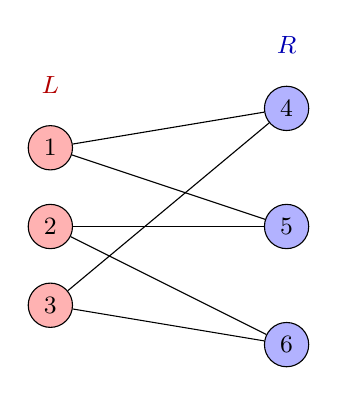
\begin{tikzpicture}[
  vertex/.style={circle, draw, minimum size=16pt, inner sep=0pt, font=\small},
  lvert/.style={vertex, fill=red!30},
  rvert/.style={vertex, fill=blue!30}
]
  % Left side
  \node[lvert] (l1) at (0,3)  {1};
  \node[lvert] (l2) at (0,2)  {2};
  \node[lvert] (l3) at (0,1)  {3};
  % Right side
  \node[rvert] (r1) at (3,3.5) {4};
  \node[rvert] (r2) at (3,2)   {5};
  \node[rvert] (r3) at (3,0.5) {6};

  \draw (l1) -- (r1);
  \draw (l1) -- (r2);
  \draw (l2) -- (r2);
  \draw (l2) -- (r3);
  \draw (l3) -- (r1);
  \draw (l3) -- (r3);

  % Labels
  \node[font=\small, red!70!black] at (0,3.8) {$L$};
  \node[font=\small, blue!70!black] at (3,4.3) {$R$};
\end{tikzpicture}
\caption{A bipartite graph with sides $L = \{1,2,3\}$ (red) and $R = \{4,5,6\}$ (blue). All edges cross between sides.}
\label{fig:bipartite}
\end{figure}

\begin{lemma}[Walk Parity]
\label{lem:walk-parity}
In a bipartite graph $(L, R)$, if a walk of length $\ell$ starts at a vertex in $L$, then it ends in $L$ if $\ell$ is even, and in $R$ if $\ell$ is odd (and symmetrically for walks starting in $R$).
\end{lemma}

\begin{proof}
By induction on the walk. Each step crosses from $L$ to $R$ or vice versa (since both sides are independent sets), toggling the parity.
\end{proof}

\begin{definition}[Bicolor]
Given a bipartition $(L, R)$ and two colors $c_1 \neq c_2$:
$\texttt{bicolor}(L, R, c_1, c_2) = \Munion(\texttt{constant\_color}(L, c_1), \texttt{constant\_color}(R, c_2))$.
\end{definition}

\begin{theorem}[Bipartite $\iff$ 2-Colorable]
\label{thm:bip-iff-2col}
For an undirected graph $g$: $g$ is bipartite if and only if there exists a complete 2-coloring of $g$.
\end{theorem}

\begin{proof}
($\Rightarrow$) Given a bipartition $(L, R)$, the bicolor construction yields a complete valid 2-coloring: vertices in $L$ get color $c_1$, vertices in $R$ get $c_2$; independence of each side ensures properness.

($\Leftarrow$) Given a complete 2-coloring $f$ with palette $\{c_1, c_2\}$, define $L = \{v \mid f(v) = c_1\}$ and $R = \nodes(g) \setminus L$. Since $f$ is proper, both sides are independent.
\end{proof}

\begin{theorem}[Neighborhoods of 3-Colorable Graphs are Bipartite]
\label{thm:nbd-bipartite}
Let $g$ be an undirected graph with a complete 3-coloring $(f, P)$. Then for every vertex $v$, the neighborhood $\texttt{neighborhood}(g, v)$ is bipartite.
\end{theorem}

\begin{proof}
If $v \notin g$, the neighborhood is empty and trivially bipartite. Otherwise, $f(v) = c$ for some color $c \in P$. Since $|P| = 3$, removing $c$ leaves a 2-element palette $P' = P \setminus \{c\}$. The restriction of $f$ to the neighborhood avoids color $c$ (by properness of $f$ across the edges from $v$ to its neighbors), yielding a complete 2-coloring of the neighborhood. By Theorem~\ref{thm:bip-iff-2col}, the neighborhood is bipartite.
\end{proof}

\begin{figure}[ht]
\centering
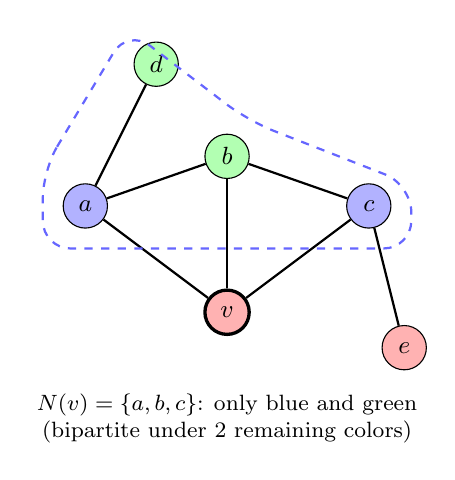
\begin{tikzpicture}[
  vertex/.style={circle, draw, minimum size=16pt, inner sep=0pt, font=\small},
  scale=0.9
]
  \node[vertex, fill=red!30, very thick]   (v)  at (0,0)   {$v$};
  \node[vertex, fill=blue!30]  (a) at (-2,1.5) {$a$};
  \node[vertex, fill=green!30] (b) at (0,2.2)  {$b$};
  \node[vertex, fill=blue!30]  (c) at (2,1.5)  {$c$};
  \node[vertex, fill=green!30] (d) at (-1,3.5)   {$d$};
  \node[vertex, fill=red!30]   (e) at (2.5,-0.5) {$e$};

  \draw[thick] (v) -- (a);
  \draw[thick] (v) -- (b);
  \draw[thick] (v) -- (c);
  \draw[thick] (a) -- (b);
  \draw[thick] (a) -- (d);
  \draw[thick] (b) -- (c);
  \draw[thick] (c) -- (e);

  % Highlight neighborhood
  \draw[dashed, blue!60, thick, rounded corners=10pt]
    ($(a)+(-0.6,0.5)$) -- ($(d)+(-0.4,0.5)$) -- ($(b)+(0.3,0.5)$) -- ($(c)+(0.6,0.3)$) -- ($(c)+(0.6,-0.6)$) -- ($(a)+(-0.6,-0.6)$) -- cycle;

  \node[font=\footnotesize, align=center] at (0,-1.5) {$N(v) = \{a, b, c\}$: only blue and green\\(bipartite under 2 remaining colors)};
\end{tikzpicture}
\caption{In a 3-colored graph, vertex $v$ (red) has neighbors using only the other two colors (blue, green), making the neighborhood bipartite.}
\label{fig:nbd-bipartite}
\end{figure}

%% ====================================================================
\section{BFS-Based 2-Coloring of Bipartite Graphs}
\label{sec:forcing}

We now describe an algorithm that, given a bipartite graph, constructs a valid 2-coloring by BFS-based layer expansion.

\subsection{Neighborhood of a Set}

\begin{definition}
For a graph $g$ and set $s$, the \emph{neighborhood of the set} is:
$\nbs(g, s) = \bigcup_{v \in s} \adj(g, v)$.
\end{definition}

\begin{lemma}
\label{lem:nbs-spec}
$i \in \nbs(g, s) \iff \exists v \in s,\; i \in \adj(g, v)$.
\end{lemma}

\subsection{Force Layers}

\begin{definition}[Force Layers]
$\texttt{force\_layers}(g, L, R, F_L, F_R, k)$ iteratively expands two frontier sets, alternating BFS layers:
\begin{itemize}[nosep]
  \item Compute $R_{\text{add}} = \nbs(g, F_L) \setminus (L \cup R)$ (new right-side vertices).
  \item Compute $L_{\text{add}} = \nbs(g, F_R) \setminus (L \cup R)$ (new left-side vertices).
  \item Recurse with updated sets $L \cup L_{\text{add}}$, $R \cup R_{\text{add}}$, and the new frontiers.
  \item Stop after $k$ iterations (where $k = |\nodes(g)|$ suffices for convergence).
\end{itemize}
\end{definition}

\begin{definition}[Force Component, Force All]
$\texttt{force\_component}(g, \text{seed}, c_1, c_2)$ runs $\texttt{force\_layers}$ from a seed vertex, then 2-colors the resulting $(L, R)$ using $\texttt{bicolor}$.

$\texttt{force\_all}(g, c_1, c_2)$ iterates: pick any vertex as seed, 2-color its connected component, remove those vertices, and recurse.
\end{definition}

\begin{figure}[ht]
\centering
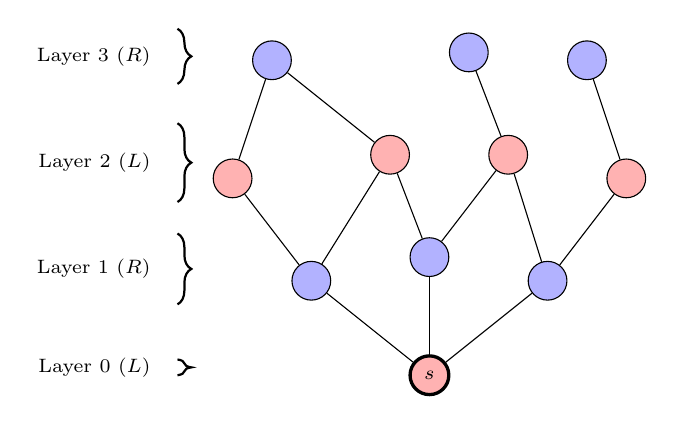
\begin{tikzpicture}[
  vertex/.style={circle, draw, minimum size=14pt, inner sep=0pt, font=\scriptsize},
  lvert/.style={vertex, fill=red!30},
  rvert/.style={vertex, fill=blue!30},
  >=Stealth
]
  % Seed
  \node[lvert, very thick] (s) at (0,0) {$s$};

  % Layer 1 (R)
  \node[rvert] (r1) at (-1.5,1.2) {};
  \node[rvert] (r2) at (0,1.5)    {};
  \node[rvert] (r3) at (1.5,1.2)  {};

  % Layer 2 (L)
  \node[lvert] (l1) at (-2.5,2.5) {};
  \node[lvert] (l2) at (-0.5,2.8) {};
  \node[lvert] (l3) at (1,2.8)    {};
  \node[lvert] (l4) at (2.5,2.5)  {};

  % Layer 3 (R)
  \node[rvert] (r4) at (-2,4) {};
  \node[rvert] (r5) at (0.5,4.1) {};
  \node[rvert] (r6) at (2,4) {};

  \draw (s) -- (r1); \draw (s) -- (r2); \draw (s) -- (r3);
  \draw (r1) -- (l1); \draw (r1) -- (l2);
  \draw (r2) -- (l2); \draw (r2) -- (l3);
  \draw (r3) -- (l3); \draw (r3) -- (l4);
  \draw (l1) -- (r4); \draw (l2) -- (r4);
  \draw (l3) -- (r5); \draw (l4) -- (r6);

  % Layer labels
  \draw[decorate, decoration={brace, amplitude=5pt, mirror}, thick]
    (-3.2,0) -- (-3.2,0.2) node[midway, left=6pt, font=\scriptsize] {Layer 0 ($L$)};
  \draw[decorate, decoration={brace, amplitude=5pt, mirror}, thick]
    (-3.2,0.9) -- (-3.2,1.8) node[midway, left=6pt, font=\scriptsize] {Layer 1 ($R$)};
  \draw[decorate, decoration={brace, amplitude=5pt, mirror}, thick]
    (-3.2,2.2) -- (-3.2,3.2) node[midway, left=6pt, font=\scriptsize] {Layer 2 ($L$)};
  \draw[decorate, decoration={brace, amplitude=5pt, mirror}, thick]
    (-3.2,3.7) -- (-3.2,4.4) node[midway, left=6pt, font=\scriptsize] {Layer 3 ($R$)};
\end{tikzpicture}
\caption{BFS layers expanding from seed $s$. Even layers (0, 2) are assigned to $L$ (red), odd layers (1, 3) to $R$ (blue). In a bipartite graph, this respects the true bipartition.}
\label{fig:bfs-layers}
\end{figure}

\subsection{Key Invariants}

\begin{lemma}[Layers Respect Bipartition]
\label{lem:layers-partition}
If $g$ has a bipartition $(B_L, B_R)$ and the seed lies in $B_L$, then after forcing, $L \subseteq B_L$ and $R \subseteq B_R$.
\end{lemma}

\begin{proof}
By induction on the number of BFS iterations. The initial state satisfies $\{\text{seed}\} \subseteq B_L$ and $\emptyset \subseteq B_R$. At each step, neighbors of left-frontier vertices land in $B_R$ (since $B_L$ is independent), and vice versa.
\end{proof}

\begin{lemma}[Reached Set is Closed]
\label{lem:reached-closed}
For an undirected bipartite graph $g$ with seed $\in \nodes(g)$:
$\nbs(g, \texttt{reached}(g, \text{seed})) \subseteq \texttt{reached}(g, \text{seed})$.
\end{lemma}

\begin{proof}
After sufficiently many BFS iterations (bounded by $|\nodes(g)|$), no new vertices are discovered. The reached set is then closed under adjacency, since any undiscovered neighbor would have been added during expansion.
\end{proof}

\begin{lemma}[Force Component OK]
\label{lem:force-comp-ok}
$\texttt{force\_component}(g, \text{seed}, c_1, c_2)$ produces a complete valid 2-coloring of the induced subgraph on the reached vertices.
\end{lemma}

\subsection{Combining Components}

\begin{lemma}[Coloring Union with No Cross Edges]
\label{lem:col-union}
Let $S \subseteq V(g)$ be closed under adjacency ($\nbs(g, S) \subseteq S$). If $f_1$ is a valid coloring of $\texttt{subgraph\_of}(g, S)$ with $\Mdomain(f_1) = S$, and $f_2$ is a valid coloring of $\texttt{remove\_nodes}(g, S)$, then $\Munion(f_1, f_2)$ is a valid coloring of $g$.
\end{lemma}

\begin{proof}
For any edge $(i,j)$ in $g$, either both endpoints are in $S$ (handled by $f_1$), or both are outside $S$ (handled by $f_2$). The closure property prevents cross-component edges.
\end{proof}

\begin{theorem}[Force All Correctness]
\label{thm:force-all}
For an undirected bipartite graph $g$ with $c_1 \neq c_2$,
the coloring $\texttt{force\_all}(g, c_1, c_2)$ is valid for $g$ with palette~$\{c_1, c_2\}$.
\end{theorem}

\begin{proof}
By well-founded induction on $|V(g)|$. At each step, $\texttt{force\_component}$ correctly 2-colors the reached set (Lemma~\ref{lem:force-comp-ok}), which is closed under adjacency (Lemma~\ref{lem:reached-closed}). By Lemma~\ref{lem:col-union}, the union with the recursive coloring of the reduced graph is valid. Bipartiteness is preserved under vertex removal. Termination follows because the reached set is non-empty (it contains the seed), so the graph strictly shrinks.
\end{proof}

%% ====================================================================
\section{Wigderson's Algorithm}
\label{sec:wigderson}

\subsection{Phase 1: High-Degree Vertex Processing}

\begin{definition}[Two-Color Neighborhood]
\[
  \texttt{two\_color\_nbd}(g, v, c_1, c_2) = \texttt{force\_all}(\texttt{neighborhood}(g, v), c_1, c_2).
\]
\end{definition}

This uses the BFS-based 2-coloring from Section~\ref{sec:forcing} on the (bipartite) neighborhood.

\begin{definition}[Phase 1]
Given a degree threshold $k$ and starting color $c$:
\begin{algorithmic}[1]
\Function{phase1}{$k, c, g$}
  \If{$\exists v \in g$ with $\degree(v, g) > k$}
    \State $m' \gets \texttt{two\_color\_nbd}(g, v, c{+}1, c{+}2)$
    \State $g' \gets \texttt{remove\_nodes}(g, \{v\} \cup \nodes(\texttt{neighborhood}(g, v)))$
    \State $(f_2, g_2) \gets \texttt{phase1}(k, c{+}3, g')$
    \State \Return $(\Munion(\{v \mapsto c\} \cup m',\; f_2),\; g_2)$
  \Else
    \State \Return $(\emptyset,\; g)$
  \EndIf
\EndFunction
\end{algorithmic}
Termination is by strict decrease of $|V(g)|$: each step removes $v$ and its neighborhood.
\end{definition}

The key feature is that colors increment by 3 at each recursive step: vertex $v$ gets color $c$, its neighbors get colors $c{+}1$ and $c{+}2$, and the next step starts from $c{+}3$. This ensures complete separation between coloring steps.

\begin{lemma}[Color Lower Bound]
\label{lem:phase1-lower}
If $\texttt{phase1}(k, c, g)$ assigns color $c_i$ to vertex $i$, then $c_i \ge c$.
\end{lemma}

\begin{proof}
By induction on $|V(g)|$. In the current step, colors $c$, $c{+}1$, $c{+}2$ are used (all $\ge c$). The recursive call starts at $c{+}3$, and by the inductive hypothesis, all colors it produces are $\ge c{+}3 > c$.
\end{proof}

\begin{theorem}[Phase 1 Coloring OK]
\label{thm:phase1-ok}
If $g$ is undirected, irreflexive, and admits a complete 3-coloring, then for any edge $(i,j)$ in $g$, if both $i$ and $j$ are colored by $\texttt{phase1}(k, c, g)$, they receive distinct colors.
\end{theorem}

\begin{proof}
By induction on $|V(g)|$. For an edge $(i,j)$, the coloring of each endpoint comes from either the current step or the recursive call. There are four cases:

\begin{enumerate}[nosep]
  \item \emph{Both current step:} If both $i$ and $j$ are colored in the same step, they are either (a)~the center $v$ and a neighbor (colors $c$ vs.\ $c{+}1$ or $c{+}2$, hence distinct), or (b)~both neighbors, handled by the correctness of \texttt{force\_all} on the bipartite neighborhood (Theorem~\ref{thm:force-all} and Theorem~\ref{thm:nbd-bipartite}).

  \item \emph{Current step and recursive call:} The current step uses colors $\le c{+}2$, while the recursive call uses colors $\ge c{+}3$ (Lemma~\ref{lem:phase1-lower}). Hence the colors differ.

  \item \emph{Recursive call and current step:} Symmetric to case 2.

  \item \emph{Both recursive:} The edge $(i,j)$ persists in the reduced graph $g'$ (since neither endpoint was removed), and the 3-coloring restricts to $g'$. The inductive hypothesis applies.
\end{enumerate}
\end{proof}

\begin{lemma}[Phase 1 Structural Properties]
\label{lem:phase1-structure}
For any undirected graph $g$:
\begin{enumerate}[nosep]
  \item The residual graph $g_2$ from $\texttt{phase1}(k, c, g)$ is a subgraph of $g$.
  \item $g_2$ is undirected and irreflexive.
  \item $g_2$ has no vertex with degree exceeding $k$.
  \item Edges between surviving vertices are preserved in $g_2$.
\end{enumerate}
\end{lemma}

\subsection{Phase 2: Degree-Bounded Greedy Coloring}

Phase 2 operates on the residual graph, which has bounded maximum degree.

\begin{definition}[Phase 2]
\begin{algorithmic}[1]
\Function{phase2}{$g$}
  \If{$\maxdeg(g) = 0$}
    \State \Return $(\texttt{constant\_color}(\nodes(g), 1),\; \emptyset)$
  \Else
    \State $d \gets \maxdeg(g)$
    \State $(s, g') \gets \texttt{extract\_vertices\_degs}(g, d)$ \Comment{independent set of max-degree vertices}
    \State $(f', g'') \gets \texttt{phase2}(g')$
    \State \Return $(\Munion(\texttt{constant\_color}(s, d{+}1),\; f'),\; g'')$
  \EndIf
\EndFunction
\end{algorithmic}
\end{definition}

At each step, the vertices of maximum degree form an independent set (Theorem~\ref{thm:max-deg-extraction}), so they can all receive the same color. The maximum degree strictly decreases after extraction, so the recursion terminates and uses at most $\maxdeg(g) + 1$ distinct colors.

\begin{theorem}[Phase 2 Correctness]
\label{thm:phase2-ok}
For any undirected irreflexive graph $g$, $\texttt{phase2}(g)$ produces a valid coloring.
\end{theorem}

\begin{proof}
By functional induction on $\texttt{phase2}$. The base case ($\maxdeg = 0$) is vacuous---no edges exist. In the step case, the independent set $s$ is colored with a fresh color $d{+}1$ not used by the recursive coloring (which uses colors corresponding to the smaller maximum degree of $g'$). The union of an independent-set coloring with a valid coloring, using a fresh color, is valid (proved as lemma \texttt{indep\_set\_union}).
\end{proof}

\subsection{The Full Algorithm}

\begin{definition}[Wigderson's Algorithm]
\label{def:wigderson}
Given a degree threshold $k$ and graph $g$:
\begin{algorithmic}[1]
\Function{wigderson}{$k, g$}
  \State $(f_1, g') \gets \texttt{phase1}(k, 1, g)$
  \State $\text{offset} \gets \texttt{max\_color}(f_1)$
  \State $f_2 \gets \texttt{phase2}(g')$
  \State \Return $\Munion(f_1, \;\text{map}\;(\lambda c.\; \text{offset} + c)\; f_2)$
\EndFunction
\end{algorithmic}
The offset ensures phase~2 colors are strictly larger than all phase~1 colors.
\end{definition}

\begin{figure}[ht]
\centering
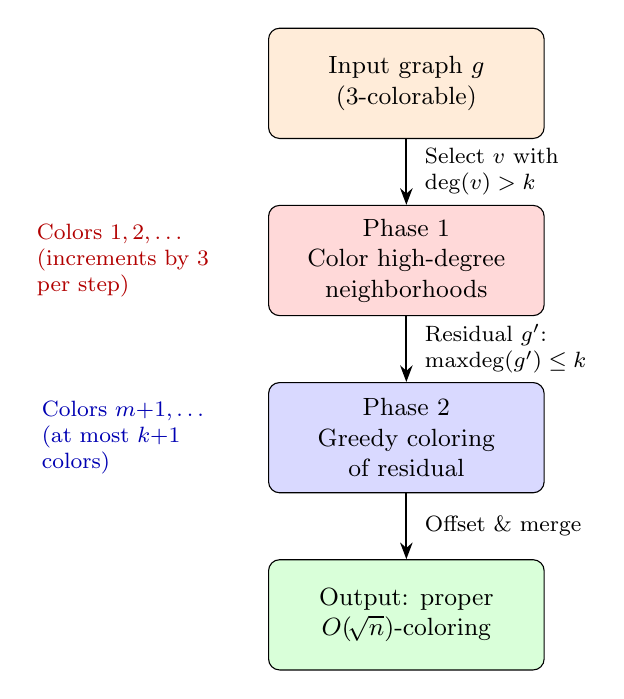
\begin{tikzpicture}[
  box/.style={rectangle, draw, rounded corners, minimum width=3.5cm, minimum height=1.4cm, align=center, font=\small},
  arr/.style={-{Stealth[length=6pt]}, thick},
  scale=0.9
]
  \node[box, fill=orange!15] (input) at (0,0) {Input graph $g$\\(3-colorable)};
  \node[box, fill=red!15]    (ph1)   at (0,-2.5) {Phase 1\\Color high-degree\\neighborhoods};
  \node[box, fill=blue!15]   (ph2)   at (0,-5) {Phase 2\\Greedy coloring\\of residual};
  \node[box, fill=green!15]  (out)   at (0,-7.5) {Output: proper\\$O(\!\sqrt{n})$-coloring};

  \draw[arr] (input) -- (ph1) node[midway, right=3pt, font=\footnotesize, align=left] {Select $v$ with\\$\degree(v) > k$};
  \draw[arr] (ph1)   -- (ph2) node[midway, right=3pt, font=\footnotesize, align=left] {Residual $g'$:\\$\maxdeg(g') \le k$};
  \draw[arr] (ph2)   -- (out) node[midway, right=3pt, font=\footnotesize] {Offset \& merge};

  % Side annotations
  \node[font=\footnotesize, align=left, text=red!70!black] at (-4,-2.5) {Colors $1, 2, \ldots$\\(increments by 3\\per step)};
  \node[font=\footnotesize, align=left, text=blue!70!black] at (-4,-5) {Colors $m{+}1, \ldots$\\(at most $k{+}1$\\colors)};
\end{tikzpicture}
\caption{Overview of Wigderson's algorithm. Phase~1 processes high-degree vertices, removing each along with its neighborhood. Phase~2 colors the bounded-degree residual. Color offsets prevent conflicts.}
\label{fig:wigderson-overview}
\end{figure}

\begin{definition}[Max Color]
$\texttt{max\_color}(f) = \texttt{fold}\;(\lambda\, k\, v\, a.\; \max(v, a))\; f\; 1$, computing the largest color value in $f$.
\end{definition}

\begin{lemma}
\label{lem:max-color}
For any $i$ with $f(i) = c_i$: $c_i \le \texttt{max\_color}(f)$.
\end{lemma}

\begin{theorem}[Wigderson Correctness]
\label{thm:wigderson-ok}
Let $g$ be an undirected, irreflexive graph with a complete 3-coloring. Then for any edge $(i,j)$ in $g$,
if $\texttt{wigderson}(k, g)$ assigns colors $c_i$ and $c_j$ to $i$ and $j$ respectively, then $c_i \neq c_j$.
\end{theorem}

\begin{proof}
Let $f_1$ be the phase~1 coloring, $f_2'$ the offset phase~2 coloring, and $w = \Munion(f_1, f_2')$ the combined result. For an edge $(i,j)$, we analyze four cases based on which map provides each color:

\begin{enumerate}[nosep]
  \item \emph{Both from $f_1$:} Apply Theorem~\ref{thm:phase1-ok}.

  \item \emph{$i$ from $f_1$, $j$ from $f_2'$:} We have $c_i \le \texttt{max\_color}(f_1) = \text{offset}$ by Lemma~\ref{lem:max-color}, while $c_j = \text{offset} + c_j^0$ for some $c_j^0 \ge 1$, so $c_j > c_i$.

  \item \emph{$i$ from $f_2'$, $j$ from $f_1$:} Symmetric to case~2.

  \item \emph{Both from $f_2'$:} Then $c_i = \text{offset} + c_i^0$ and $c_j = \text{offset} + c_j^0$. Since $i$ and $j$ are both in the residual graph $g'$ and the edge persists in $g'$ (Lemma~\ref{lem:phase1-structure}), Phase~2 assigns $c_i^0 \neq c_j^0$ (Theorem~\ref{thm:phase2-ok}), hence $c_i \neq c_j$ by injectivity of the offset.
\end{enumerate}
\end{proof}

\subsection{Color Complexity}

We now prove that, with an appropriate choice of threshold, the algorithm uses
$O(\!\sqrt{n})$ colors.
We begin by bounding the number of colors used by each phase separately.

\begin{lemma}[Phase~1 Iteration Count]
\label{lem:phase1-steps}
Let $g$ be an undirected irreflexive graph on $n$~vertices, and let $k$~be the
degree threshold.
Phase~1 performs at most $\lfloor n/(k{+}2) \rfloor$ iterations.
\end{lemma}

\begin{proof}
At each iteration, a vertex~$v$ with $\degree(v,g) > k$ is selected.
The algorithm removes the set $\{v\} \cup \adj(g,v)$ from the current graph.
Since $g$ is irreflexive, $v \notin \adj(g,v)$, so
$|\{v\} \cup \adj(g,v)| = 1 + |\adj(g,v)| \ge 1 + (k{+}1) = k{+}2$.

Successive iterations remove disjoint subsets of the original vertex set
(each iteration removes vertices from the current graph,
which excludes all previously removed vertices).
If phase~1 performs $t$~iterations, then $t \cdot (k{+}2) \le n$,
giving $t \le \lfloor n/(k{+}2)\rfloor$.
\end{proof}

\begin{lemma}[Phase~1 Color Count]
\label{lem:phase1-colors}
Phase~1 uses at most $3\lfloor n/(k{+}2)\rfloor$ distinct colors.
More precisely, $\texttt{max\_color}(f_1) \le 3\lfloor n/(k{+}2)\rfloor$.
\end{lemma}

\begin{proof}
At the $i$-th iteration ($i = 1, 2, \ldots, t$), the starting color parameter is
$c = 1 + 3(i{-}1)$.
The three colors used are $c$, $c{+}1$, $c{+}2$, \ie, $3i{-}2$, $3i{-}1$, $3i$.
After $t$~iterations the largest color is~$3t$.
By Lemma~\ref{lem:phase1-steps}, $t \le \lfloor n/(k{+}2)\rfloor$,
so the maximum color is at most $3\lfloor n/(k{+}2)\rfloor$.
\end{proof}

\begin{lemma}[Phase~2 Color Count]
\label{lem:phase2-colors}
Let $g'$ be the residual graph after phase~1.
Phase~2 uses at most $\maxdeg(g') + 1$ distinct colors.
\end{lemma}

\begin{proof}
Phase~2 proceeds by repeatedly extracting the independent set of
maximum-degree vertices and assigning them a single fresh color.
At each step the maximum degree strictly decreases
(by Theorem~\ref{thm:max-deg-extraction} and the exhaustion lemma).
Starting from $\maxdeg(g') = d$, the algorithm uses one color for
degree~$d$, one for degree~$d{-}1$, and so on down to degree~$0$
(whose vertices all receive color~$1$).
This gives exactly $d + 1$ colors, numbered $1, 2, \ldots, d{+}1$.

More precisely, the Coq proof establishes
(via \texttt{phase2\_color\_bound})
that every color $c$ assigned by phase~2 satisfies
$c \le \maxdeg(g') + 1$ when expressed as a natural number.
\end{proof}

\begin{theorem}[Color Bound --- \texttt{wigderson\_color\_bound}]
\label{thm:color-bound}
Let $g$ be an undirected irreflexive graph on $n$~vertices.
With degree threshold $k \ge 0$, every color~$c_i$ assigned by
$\texttt{wigderson}(k, g)$ satisfies
\[
  c_i \;\le\; 3\!\left\lfloor \frac{n}{k+2} \right\rfloor + k + 2.
\]
In particular, setting $k = \lfloor\!\sqrt{n}\rfloor$ gives
$O(\!\sqrt{n})$ colors.
\end{theorem}

\begin{proof}
Let $(f_1, g') = \texttt{phase1}(k, 1, g)$ and $f_2 = \texttt{phase2}(g')$.
Let $m = \texttt{max\_color}(f_1)$.
The combined coloring is
\[
  w = \Munion\!\bigl(f_1,\; \text{map}\;(\lambda c.\; m + c)\; f_2\bigr).
\]
For any vertex~$i$ with $w(i) = c_i$, we case-split on whether $c_i$ comes from~$f_1$ or the shifted~$f_2$.

\medskip\noindent
\textbf{Phase~1 colors.}
We prove inductively (\texttt{phase1\_color\_upper\_bound}) that every color $c_i$ assigned by $\texttt{phase1}(k, c, g)$ satisfies
$c_i + 1 \le c + 3\lfloor |V(g)|/(k{+}2) \rfloor$.
The induction is on $|V(g)|$ using well-founded induction.
In the step case, a high-degree vertex~$v$ is selected; the current step uses colors $c, c{+}1, c{+}2$, which are all $\le c + 2$.
Since $v$ has degree $> k$, removing $\{v\} \cup \adj(g,v)$ decreases the vertex count by at least $k{+}2$ (\texttt{phase1\_removes\_many}).
This yields $\lfloor |V(g')|/(k{+}2)\rfloor + 1 \le \lfloor |V(g)|/(k{+}2)\rfloor$ by integer division (\texttt{nat\_div\_step}),
allowing the inductive bound on colors from the recursive call to be absorbed.

With $c = 1$: $c_i + 1 \le 1 + 3\lfloor n/(k{+}2)\rfloor$, so $c_i \le 3\lfloor n/(k{+}2)\rfloor \le 3\lfloor n/(k{+}2)\rfloor + k + 2$.

\medskip\noindent
\textbf{Phase~2 colors.}
If $c_i = m + c_i^0$ for some phase~2 color~$c_i^0$, we bound each term:
\begin{itemize}[nosep]
  \item \emph{Bounding~$m$:}
  By \texttt{max\_color\_bound\_nat} and the phase~1 bound above,
  $m \le 3\lfloor n/(k{+}2)\rfloor + 1$.
  (The $+1$ accounts for the base case where $f_1$ is empty and $m = 1$.)
  \item \emph{Bounding~$c_i^0$:}
  By \texttt{phase2\_color\_bound}, $c_i^0 \le \maxdeg(g') + 1$.
  By \texttt{phase1\_residual\_max\_deg}, the residual graph has $\maxdeg(g') \le k$
  (no high-degree vertices remain after phase~1).
  Hence $c_i^0 \le k + 1$.
\end{itemize}
Combining: $c_i = m + c_i^0 \le (3\lfloor n/(k{+}2)\rfloor + 1) + (k + 1) = 3\lfloor n/(k{+}2)\rfloor + k + 2$.

\medskip\noindent
\textbf{Asymptotic bound.}
Setting $k = \lfloor\!\sqrt{n}\rfloor$:
\[
  3\!\left\lfloor \frac{n}{\lfloor\!\sqrt{n}\rfloor + 2} \right\rfloor
  + \lfloor\!\sqrt{n}\rfloor + 2
  \;\le\;
  \frac{3n}{\sqrt{n}}
  + \sqrt{n} + 2
  \;=\;
  4\sqrt{n} + 2,
\]
which is $O(\!\sqrt{n})$.
\end{proof}

\begin{remark}
The constant can be improved by optimizing the threshold.
Setting $k = \lfloor\!\sqrt{3n}\rfloor - 2$ minimizes the expression
$3n/(k{+}2) + k + 2$, yielding an upper bound of approximately
$2\sqrt{3n} + 2 \approx 3.47\sqrt{n}$ colors.
However, the standard statement of Wigderson's result simply asserts
$O(\!\sqrt{n})$, which our proof establishes.
The Coq theorem (\texttt{wigderson\_color\_bound}) states this bound
directly on each color value, requiring only undirectedness and
irreflexivity as preconditions---notably, 3-colorability is not needed
for the bound itself, only for correctness.
\end{remark}

\begin{corollary}[Asymptotic Bound --- \texttt{wigderson\_sqrt\_bound}]
\label{cor:sqrt-bound}
Let $g$ be an undirected irreflexive graph on $n$~vertices.
Setting $k = \lfloor\!\sqrt{n}\rfloor$, every color~$c_i$ assigned by
$\texttt{wigderson}(\lfloor\!\sqrt{n}\rfloor, g)$ satisfies
\[
  c_i \;\le\; 4\lfloor\!\sqrt{n}\rfloor + 2.
\]
\end{corollary}

\begin{proof}
By Theorem~\ref{thm:color-bound} with $k = \lfloor\!\sqrt{n}\rfloor$,
it suffices to show $3\lfloor n/(\lfloor\!\sqrt{n}\rfloor + 2)\rfloor \le 3\lfloor\!\sqrt{n}\rfloor$,
\ie, $\lfloor n/(\lfloor\!\sqrt{n}\rfloor + 2)\rfloor \le \lfloor\!\sqrt{n}\rfloor$.
This holds because $n \le \lfloor\!\sqrt{n}\rfloor \cdot (\lfloor\!\sqrt{n}\rfloor + 2)$,
which follows from $n < (\lfloor\!\sqrt{n}\rfloor + 1)^2 = \lfloor\!\sqrt{n}\rfloor^2 + 2\lfloor\!\sqrt{n}\rfloor + 1$
(the defining property of the integer square root).
In Coq, the key step uses \texttt{Nat.sqrt\_spec} and nonlinear arithmetic (\texttt{nia}).
\end{proof}

%% ====================================================================
\section{Conclusion}
\label{sec:conclusion}

We have presented a complete formal verification of Wigderson's graph coloring algorithm in Coq. The main results are: (1)~the algorithm produces a proper coloring of any 3-colorable undirected graph (\texttt{wigderson\_ok}, Theorem~\ref{thm:wigderson-ok}), (2)~every color assigned is bounded by $3\lfloor n/(k{+}2)\rfloor + k + 2$ (\texttt{wigderson\_color\_bound}, Theorem~\ref{thm:color-bound}), and (3)~setting $k = \lfloor\!\sqrt{n}\rfloor$ yields the concrete bound $c_i \le 4\lfloor\!\sqrt{n}\rfloor + 2$ (\texttt{wigderson\_sqrt\_bound}, Corollary~\ref{cor:sqrt-bound}), formally establishing the $O(\!\sqrt{n})$ guarantee.

The formalization consists of approximately 6{,}600 lines of Coq across 9 source files:
\begin{itemize}[nosep]
  \item \texttt{graph.v}: Core graph definitions, domain lemmas, and greedy coloring.
  \item \texttt{restrict.v}: Map restriction by key sets.
  \item \texttt{munion.v}: Left-biased map union.
  \item \texttt{subgraph.v}: Induced subgraphs, neighborhoods, degrees, independent sets.
  \item \texttt{coloring.v}: Coloring completeness, $n$-coloring, union of disjoint colorings.
  \item \texttt{connectivity.v}: Walks, reachability, bipartition parity.
  \item \texttt{bipartite.v}: Bipartition, 2-coloring equivalence.
  \item \texttt{forcing.v}: BFS-based 2-coloring of bipartite graphs.
  \item \texttt{wigderson.v}: Both phases, the main correctness theorem, and the color bound.
\end{itemize}

The proof makes extensive use of CoqHammer~\cite{coqhammer} for automation, particularly the \texttt{hauto}, \texttt{sauto}, and \texttt{sfirstorder} tactics, which handle many routine first-order reasoning steps. All proofs are complete---no \texttt{Admitted} declarations remain.

A notable design choice is the use of Coq's \texttt{Function} command with \texttt{\{measure M.cardinal g\}} for defining recursive functions over graphs, enabling termination proofs based on the strict decrease of the vertex count. The BFS-based 2-coloring (\texttt{force\_all}) uses well-founded induction on graph cardinality, while \texttt{phase1} and \texttt{phase2} both use the \texttt{Function} mechanism.

\bigskip
\noindent\textbf{Acknowledgments.} The graph representation and greedy coloring algorithm are based on the VFA (Verified Functional Algorithms) development by Andrew Appel.

\begin{thebibliography}{9}
\bibitem{wigderson83}
A.~Wigderson.
\newblock Improving the performance guarantee for approximate graph coloring.
\newblock \emph{Journal of the ACM}, 30(4):729--735, 1983.

\bibitem{coqhammer}
\L.~Czajka and C.~Kaliszyk.
\newblock Hammer for {C}oq: Automation for dependent type theory.
\newblock \emph{Journal of Automated Reasoning}, 61(1--4):423--453, 2018.
\end{thebibliography}

\end{document}
